% !TeX root = ../../Skript.tex
\cohead{\Large\textbf{Berühren von Funktionen}}
\fakesubsection{Berühren von Funktionen}
Das Berühren zweier Funktionen \(f(x)\) und \(g(x)\) ist die Erweiterung der Tangente auf beliebige Funktionen. Eine Tangente ist eine Gerade, die eine Funktion an einer Stelle berührt. Man kann statt einer Geraden aber eine beliebige Funktion wählen. Die beiden Bedingungen, die erfüllt sein müssen, damit sich zwei Funktionen an einer Stelle \(x_0\) berühren, bleiben aber die gleichen:
\begin{tcolorbox}

    \bigskip

	\textcolor{loestc}{Die Steigungen der beiden Funktionen an der Stelle \(x_0\) müssen gleich sein:
		\[m\cdot f'(x_0)=g'(x_0)\]}
\end{tcolorbox}
\begin{tcolorbox}

    \bigskip

	\textcolor{loestc}{Die Funktionswerte der beiden Funktionen an der Stelle \(x_0\) müssen gleich sein:
		\[f(x_0)=g(x_0)\]}
\end{tcolorbox}
Beispiel: Zeige, dass sich die beiden Funktionen \(f(x)=x^3+1\) und \(g(x)=x^2+x\) in genau einem Punkt berühren.\vspace{0.5cm}

\begin{minipage}{\textwidth}
       \adjustbox{valign=t}{\begin{minipage}{0.5\textwidth+2ex}
		\begin{enumerate}
			\item Die Steigungen müssen gleich sein:
			\begin{align*}
				\textcolor{loes}{f'(x)}&\textcolor{loes}{=g'(x)}\\
				\textcolor{loes}{3x^2}&\textcolor{loes}{=2x+1\ \vert\ -2x-1}\\
				\textcolor{loes}{3x^2-2x-1}&\textcolor{loes}{=0}\\
				\textcolor{loes}{x_{1/2}}&\textcolor{loes}{=\frac{2\pm\sqrt{4-4\cdot a\cdot (-1)}}{6}}\\
				\textcolor{loes}{x_1}&\textcolor{loes}{=1\text{ und }x_2=-\tfrac{1}{3}}
			\end{align*}

            \bigskip


			\item Gleiche Funktionswerte:

			\textcolor{loes}{\(f\left(-\tfrac{1}{3}\right)=\frac{26}{27}\neq-\frac{2}{9}=g\left(-\tfrac{1}{3}\right)\)}

			\textcolor{loes}{Die beiden Funktionen berühren sich nicht bei \(x_2=-\tfrac{1}{3}\)}

			\textcolor{loes}{\(f(1)=2=g(1)\)}

			\textcolor{loes}{Die beiden Funktionen berühren sich also bei \(x_1=1\)}
		\end{enumerate}
	\end{minipage}}%
    \adjustbox{valign=t, padding=2ex 0ex 0ex 0ex}{\begin{minipage}{0.5\textwidth-4ex}
		\centering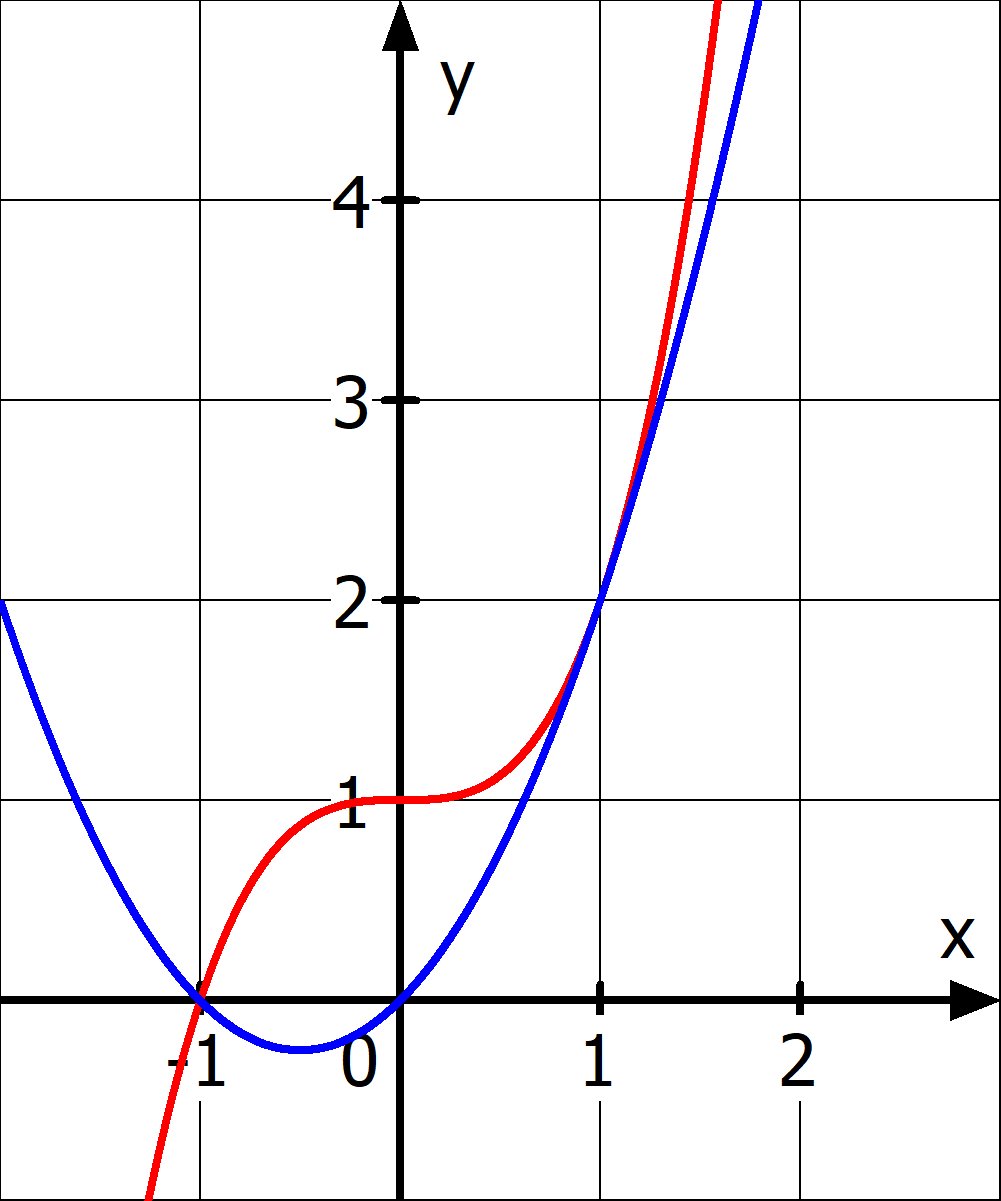
\includegraphics[width=\textwidth]{\ableitung/pics/beruehrenBsp.png}
	\end{minipage}}%
\end{minipage}

\bigskip

\textcolor{loes}{Hinweis: Man kann zuerst auf gleiche Funktionswerte oder auf gleiche Steigungen prüfen. In den allermeisten Fällen ist es einfacher zuerst auf gleiche Steigungen zu prüfen, z.B. hätte man im obigen Beispiel beim Lösen von \(f(x)=g(x)\) eine Gleichung erhalten, die wir mit unseren Methoden nicht lösen können.}\newpage
%%%%%%%%%%%%%%%%%%%%%%%%%%%%%%%%%%%%%%%%%%%%%%%%%%%%%%%%%%%%%%%%%%%%%%%%%%%%%%%%%%%%%%%%%%%%%%%%%%%%%%%
\begin{Exercise}[title={\raggedright Bestimme jeweils den Berührpunkt der beiden Funktionen.}, label=beruehrpunkteA1]
	\begin{enumerate}[label=\alph*)]
		\item \(f(x)=\frac{1}{3}x^3-x^2\) und \(g(x)=-x^2+9x-18\)
		\item \(f(x)=x^2-2x+1\) und \(g(x)=-x^2+6x-7\)
		\item \(f(x)=\frac{1}{2}x^2+4x+\frac{1}{2}\) und \(g(x)=x^3-2\)
		\item \(f(x)=x^2+2x-13\) und \(g(x)=2x^2-4x-4\)
		\item \(f(x)=\frac{1}{6}x^3-\frac{1}{6}x^2-x\) und \(g(x)=-3x^2-13,5x-16,5\)
		\item \(f(x)=x^5-x^3+2\) und \(g(x)=x^3-x+2\quad\) Hinweis: 2 Berührpunkte
		\item \(f(x)=-x^3+x+1,5\) und \(g(x)=-x^2+x+1,5\)
		\item \(f(x)=-2e^{-x}+2\) und \(g(x)=\frac{1}{2}e^x\)
		\item \(f(x)=-\frac{1}{7}e^{-x}+1\) und \(g(x)=7e^x+1\)
		\item \(f(x)=-\frac{1}{e^2}e^{-x}\) und \(g(x)=e^x-\frac{2}{e}\)
	\end{enumerate}
\end{Exercise}
%%%%%%%%%%%%%%%%%%%%%%%%%%%%%%%%%%%%%%%%%
\begin{Answer}[ref=beruehrpunkteA1]
	\begin{enumerate}[label=\alph*)]
		\item \(P(3\vert0)\)
		\item \(P(2\vert1)\)
		\item \(P(-1\vert-3)\)
		\item \(P(3\vert2)\)
		\item \(P(-3\vert-3)\)
		\item \(P(1\vert2)\) und \(Q(-1\vert2)\)
		\item \(P(0\vert1,5)\)
		\item \(P(\ln(2)\vert1)\)
		\item \(P(-2\vert0)\)
		\item \(P\left(-1\vert-\frac{1}{e}\right)\)
	\end{enumerate}
\end{Answer}